\documentclass{jsarticle}
\usepackage{amsmath,amssymb}
\usepackage{amsthm}
%\usepackage{pdfpages}
%\usepackage{mediabb}
\usepackage[dvipdfmx]{graphicx}
\usepackage{color}
%\usepackage{mediabb}
\theoremstyle{definition}
\newtheorem{theorem}{定理}
\newtheorem{definition}[theorem]{定義}
\newtheorem{lemma}[theorem]{補題}
\renewcommand\proofname{\bf 証明}
\begin{document}
\section{Shor's algorithm}
\subsection{アルゴリズムの目標}
$M \in \mathbb{Z}_{>0}$に対して, 次の$2$つの条件を満たす函数$f:\mathbb{N}\rightarrow \{0, M-1 \}$を考える.\\
【条件】\\
$1.$ 周期 $^{\exists !}r$	$($i.e$)$ for $^{\forall} x \in \mathbb{N}, $ $f(x+r)=f(x)$\\
$2.$ $f(0), \cdots , f(r-1)$ are all distinct. 

\subsection{アルゴリズムの戦略}
ここで述べるShorのアルゴリズムは, IQFTを用いない確率的なアルゴリズムである. 
まず, 記号の準備をする.
\begin{equation}
 \begin{array}{crcc}
for \hspace{5pt}a \in \mathbb{N}, \hspace{5pt} & f_a:\mathbb{N} &\rightarrow& \{ 0, \cdots , M-1 \} \\
 &x &\mapsto& a^x \mod M.
 \end{array}
 \end{equation}
Step$1.$ $M ( n$  bit $)$ の整数,  $a \in \{1, M-1 \}$ を gcd $(a, M)=1$を満たす整数とする. さらに$Q$を
\begin{equation}\label{M_condition}
M^2 \leq Q =2^{\ell} \leq 2\cdot M^2
\end{equation}
を満たす最小の$2べきの数とする.$ \\
Step $2.$ 等重の並列状態にする. $\frac{1}{\sqrt{Q} } \displaystyle\sum_{x}^{Q-1}  |x  \rangle$ \\
Step $3.$ Quantum part (後述)  return $\displaystyle\sum_x\alpha_x |x \rangle | k \rangle $\\
Step $4.$ 第一レジスタを観測する. \\
Step $5.$ 周期$r$をStep $4.$で得た数値から推定する. もしStep$4$での数値が "good number " なら, $r$を推測できる. そうでなければ,再度Step $3$に戻る.\\
\section{Good Number}
\begin{definition}
$x \in \{0, \cdots , Q-1 \}$ が " Good number "であるとは, 
\begin{equation}\label{good}
^\exists (t, r) :互いに素 \hspace{5pt} (s.t) \hspace{5pt}   t \cdot Q -x\cdot r=k   \hspace{5pt}  where \hspace{5pt}  -r/2 \leq  k \leq r/2  
\end{equation}
\end{definition}
例として, $Q=256$\\
$t=1.0, r=4, x=64,   k=0$\\
$t=3.0, r=4, x=192, k=0$\\

\begin{theorem}
$x$がGood numberの時, 連分数展開によって, 周期$r$が一意的に定まる.
\end{theorem}
\begin{proof}
Good number の定義から, 
\begin{equation}
\left| \frac{x}{Q} -\frac{t}{r} \right| \leq \frac{1}{2Q}  \leq \frac{1}{M^2} \leq \frac{1}{r^2}
\end{equation}
連分数展開について次の定理がある.
\begin{theorem}
$\frac{P}{ Q}$を$\|\frac{P}{ Q} -x \| < \frac{1}{2Q^2}$を満たす任意の有理数とする時、$\frac{P}{ Q}$は$x$の近似分数である。さらに、その近似分数は$P,Q$の最大公約数は$1$である.
\end{theorem}
\end{proof}
\begin{lemma}
There are $\Omega\left(\frac{r}{\log\log r} \right)$ good numbers.
\end{lemma}
\section{Quantum part of the Algorithm}
ここでは, Step $3$, $4$ について述べる.\\
Quantum-Step $1$.  次の量子重ね合わせ状態を構成する.\\
\begin{equation}
\frac{1}{\sqrt{Q}} \displaystyle\sum_{x=0}^{Q-1}|x\rangle \otimes |f_a (x)\rangle
\end{equation}
Quantum-Step $2$. 離散フーリエ変換 
$$\begin{array}{rcc}
\mathcal{F}_Q: \mathbb{C}^Q &\rightarrow &\mathbb{C}^Q \\
|x \rangle                               &\mapsto     &\frac{1}{\sqrt{Q}} \displaystyle\sum_{k=0}^{Q-1}\exp\left(2\pi i \frac{x\cdot k}{Q}\right) |k\rangle 
\end{array}
$$
を第一レジスタに作用させる. この時, 量子状態を 
\begin{equation}
\displaystyle\sum_{(xy) , x \in \{ 0,Q-1 \} }b(xy)| x \rangle \otimes |y\rangle
\end{equation}とする.\\
Quatnum-Step $3$. 第一レジスタを観測する.

\subsection{Analysis}
\begin{lemma}
Quantum-Step$2$について, $b(xy)$は,  $f(x_0)=y, T=1+  \lfloor \frac{Q-x_0}{r} \rfloor$ とした時, 
\begin{equation}\label{prob}
b(xy)=\omega^{x_0 +(T-1)r}\frac{1}{Q}\left( \frac{\sin (T\cdot \pi xr /Q )}{\sin (\pi x r / Q)}\right)
\end{equation}
\end{lemma}
\begin{proof}
\end{proof}
(\ref{prob})について, $x$がGood number (\ref{good}), i.e. $t Q-xr=k$の時, 
$$\begin{array}{ccc}
b(xy)&=&\omega^{x_0 +(T-1)r}\frac{1}{Q}\left( \frac{\sin (T\cdot \pi xr /Q )}{\sin (\pi x r / Q)}\right)\\
       &=&\omega^{x_0 +(T-1)r}\frac{1}{Q}\left( \frac{\sin (T\cdot \pi \frac{ tQ-xr }{ Q} )}{\sin (\pi \frac{tQ-xr}{ Q})}\right)
\end{array}
$$
$T$の定義から
\begin{equation}\label{T_cond}
T \leq 1+ \frac{Q}{r}
\end{equation}
$x$がGood number であることから,
\begin{equation}\label{alpha_cond}
-\frac{r}{2Q} \leq \frac{ tQ-xr }{ Q} =\frac{k}{Q} \leq \frac{r}{2Q}
\end{equation}
(\ref{T_cond}) ,(\ref{alpha_cond})から
\begin{equation}\label{Talpha_cond}
T\cdot \frac{ tQ-xr }{ Q} \leq \frac{1}{2}+ \frac{r}{2Q}
\end{equation} 
(\ref{M_condition})から, 
\begin{equation}
\frac{Q}{r} >\frac{M^2}{ r} > M 
\end{equation}
であることを思い出しておく. 先ほどの(\ref{Talpha_cond})から
\begin{equation}\label{main_condition}
\pi \cdot T\cdot \frac{ tQ-xr }{ Q}  \leq  \pi \left( \frac{1}{2}+ \frac{r}{2Q} \right) \leq \pi \left( \frac{1}{2}+ \frac{1}{2M}\right)
\end{equation}
ここで, 
\begin{equation}
\alpha:=\frac{ tQ-xr }{ Q}. 
\end{equation}
と置いたとき, (\ref{main_condition}) は
\begin{equation}
T\cdot \alpha \leq \pi \left( \frac{1}{2}+ \frac{1}{2M}\right)
\end{equation}
となることがわかり、よって
\begin{align}
\|b(xy)\|^2&=\left\| \frac{1}{Q} \left( \frac{ \sin (T\cdot \alpha  ) }{\sin \alpha } \right) \right\| ^2\\
        &\geq \frac{T^2}{Q^2}  \left( \frac{ \sin (T\cdot \alpha  ) }{T \alpha } \right) ^2
\end{align}
$\frac{ \sin (x  ) }{x}$を, 微分した時の分子は, $\cos x \cdot (x-\tan x)$となるため $0\leq x \leq \frac{\pi}{2}$で単調減少する.


\section{考察}
Good numberは以下の通り. $(M=15, a=2$の時 $)$ 参考: $r=4$\\
$\text{Case } 1: Q=2$の時\\
$\text{Case } 2:  Q=4$の時\\
$t=1.0, x=1, k=0 $\\
なので$ \frac{Good numberの数}{Q}=\frac{1}{4}$\\
一方で, Shorのアルゴリズムによると, $x=1$が出力される確率は$(\ref{prob})$より$\frac{1}{4}$とわかる.\\
$\text{Case } 3:  Q=8$の時 \\
$t=1.0, x=2, k=0$;\\
$t=3.0, x=6, k=0$;\\
$ \frac{Good numberの数}{Q}=\frac{1}{4}$である一方で、理論値では$\frac{3}{16}$ \\
$\text{Case } 4:  Q=16$の時 \\
$t=1.0, x=4, k=0$\\
$t=3.0, x=12, k=0$\\
$ \frac{Good numberの数}{Q}=\frac{1}{8}$である一方で、理論値では$\frac{1}{8}$ \\
$\text{Case } 5:  Q=32$の時 \\
t$=1.0, x=8, k=0$\\
$t=3.0, x=24, k=0$


\begin{figure}[h]
\begin{center}
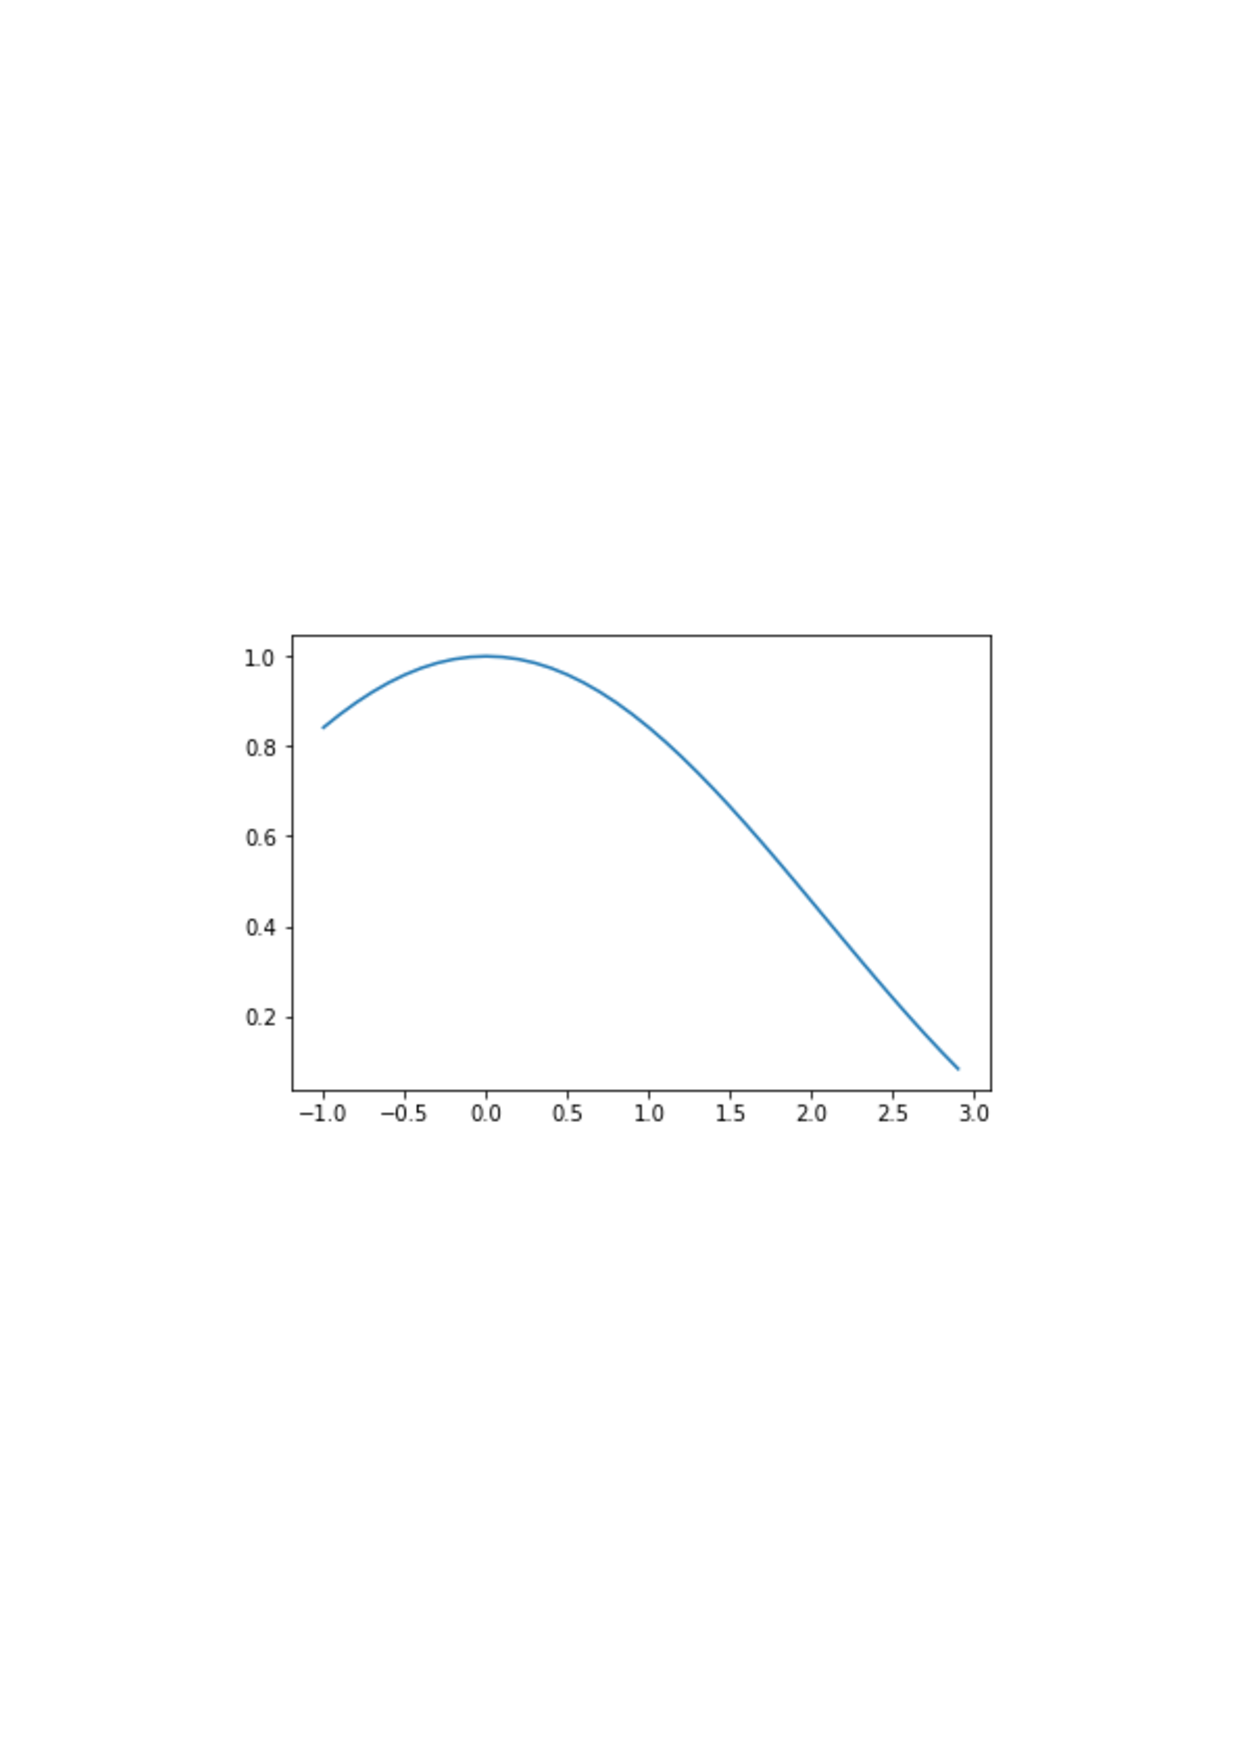
\includegraphics[width=1.0\linewidth]{sin_x_ov_x.pdf}
\caption{$\frac{sin(x)}{x}$}
%\label{ラベル}
\end{center}
\end{figure}

\section{考えたいこと}
研究$1$. サンプリングごとに$Q$を変えていってsearchする. $(ベイズ更新のように)$\\
研究$2$. 大西さんの結果とGood numberの数の関係\\

\section{RSA暗号と素因数分解問題について}
$p,q $を素数として$M=p\cdot q.$ この時, 
\begin{equation}
 \left(M/ M\mathbb{Z} \right)^{*} \simeq   \left(M/ p \mathbb{Z} \right)^{*} \times  \left(M / q \mathbb{Z} \right)^{*}.
 \end{equation}
 今, $e \in  \left( M/ M\mathbb{Z} \right)^{*} $に対して, $^ \exists e' \in  \left( M/  M\mathbb{Z} \right)^{*} $ s.t  $e\cdot e' =1 \mod (p-1)\cdot (q-1)$. ここで, $e$が公開情報, $e'$が秘密情報となる.\\
 【暗号化】\\
 メッセージ $m$ に対して $m^e$で暗号化する.\\
 復号は, $e\cdot e' =^{\exists}k\cdot (p-1)\cdot (q-1)+ 1$だから, $(m^e)^{e'}=m^{e\cdot e'}=m^{k\cdot (p-1)\cdot (q-1)+1  }=m$ となる.
 
\end{document}
